%*******************************************************************************
%*********************************** First Introduction *****************************
%*******************************************************************************
%\chapter{Introduction}  %Title of the First Introduction
%\chapter*{Introduction}
\chapter{Related Work}  %Title of the First Introduction
%\addcontentsline{tableofcontents}{chapter}{introduction}

\ifpdf
    \graphicspath{{Background/Figs/Raster/}{Background/Figs/PDF/}{Background/Figs/}}
\else
    \graphicspath{{Background/Figs/Vector/}{Background/Figs/}}
\fi
This chapter will explore the research related to this thesis. First we introduce briefly named entity recognition, an important step before relation extraction. Next different relation extraction algorithms are presented.
%********************************** %First Section  **************************************
\section{Named Entity Recognition} %Section - 2.1
\emph{Named Entity Recognition}, or NER, is the task of identifying elements in text that belong to pre-defined categories. Specifically, NER in biomedical text mining aims at identifying entities such as proteins, diseases, genes, etc. There is extra difficulty for NER in the biomedical domain mainly for the following reasons. First, there is no canonical dictionary for biomedical entities\cite{cohen2005survey}. The entity names are created on the fly and the number of names is in the millions. Second, the names are not defined unambiguously\cite{wilbur2007biocreative}. The same name may refer to different entities depending on context, in the meantime an entity might have several names. Finally, even human interpretations differ with named entities in the biomedical text. For example in our corpus for this project there were about 10\% disagreement on named entities between two human annotators\cite{verspoor2013annotating}.
%********************************** %Second Section  *************************************
\section{Relation Extraction}%Section - 2.2
While it is often the case that the accuracy of named entity recognition would have a significant impact on the performance of relation extraction, the two problems are usually treated separately. This allows the relevant tools for each problem to be evaluated independently. Therefore, in the following sections, the relation extraction methods usually have the named entity annotations given in their test data, so that the algorithm only needs to focus on extracting relations between known entities.
\subsection{Pattern Based Methods}
Pattern based relation extraction methods first saw its application in extracting protein-protein interactions\cite{hao2005discovering}. Initially, a set of part-of-speech rules are applied to split the syntactically complex sentence into simple sentences. For example, a sentence with part-of-speech tag sequence \emph{\big\{P1, VB1, P2, VB2, CC, P3\big\}} can be splitted to \emph{\big\{P1, VB1, P2\big\}} and \emph{\big\{P1, VB2, P3\big\}}. Then, a set of word patterns can be applied to extract relations from these simple sentences\cite{ono2001automated}. An example of that is shown in Figure \ref{fig:Word_Patterns}. 
	\begin{figure}
		\centering
		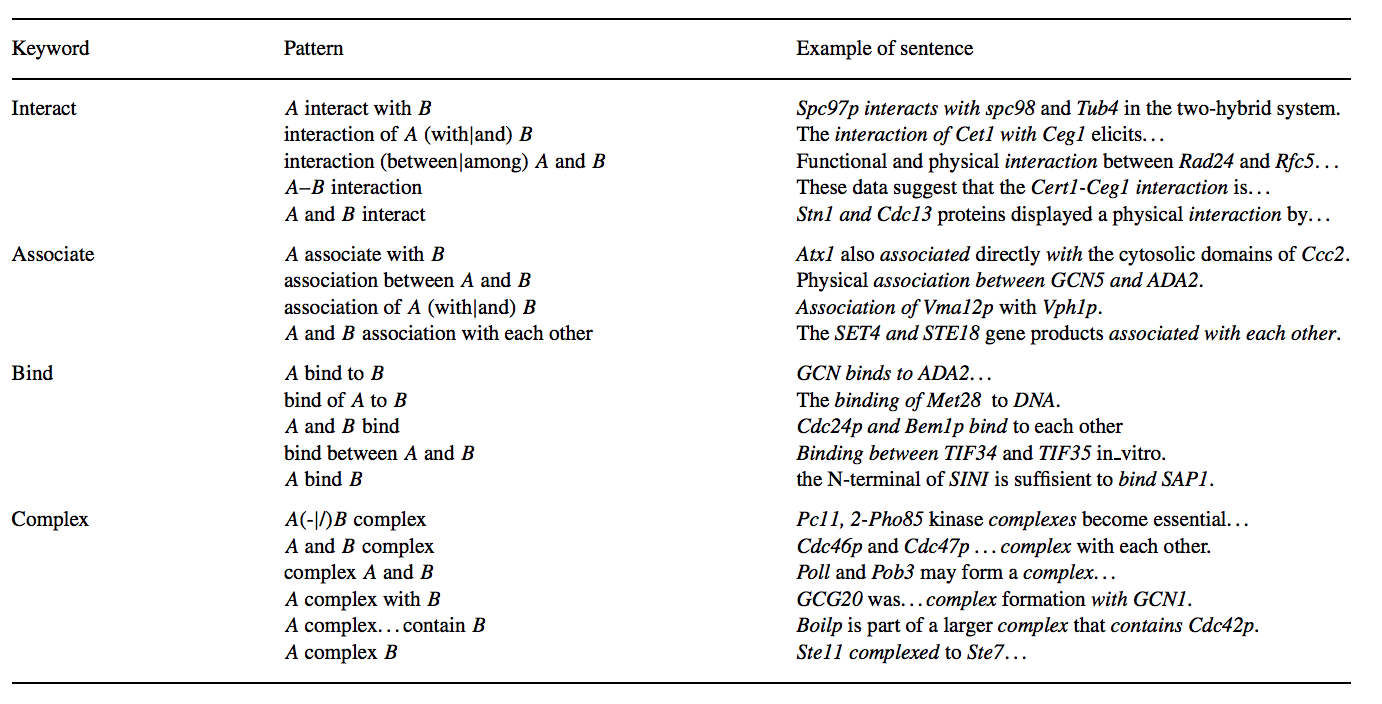
\includegraphics[width=\textwidth]{Word_Patterns}
		\caption{Word Patterns for Protein-Protein Interaction from \citet*{ono2001automated}}
		\label{fig:Word_Patterns}   
	\end{figure}
In addition, \citet{hao2005discovering} proposed an idea of minimal description length, as in finding the optimal pattern set that has the most balance among high precision, short rule length and low rule complexity by dynamic programming. Pattern based methods has achieved quite respectable performances for extracting protein-protein interactions\cite{hao2005discovering}. However, it does not incorporate the richness of expressions, such as the anaphora terms like pronouns. Consequently, it does not generalize well and usually needs huge amount of training data.
\subsection{Co-occurrence based methods}
Finding co-occurring terms within a sentence or abstract has been the foundation of many relation extraction algorithms\cite{chaussabel2002mining,becker2003pubmatrix,tanabe1999medminer,stapley2000biobibliometrics,jenssen2001literature,wren2004knowledge}. Simple co-occurrence measures include probabilistic indicators such as point-wise mutual information, chi-square and log-likelihood ratio. More advanced measures include Concept Space, where thesaurus are mapped to a multi-dimensional Euclidean space\cite{leroy2005genescene, van2004constructing}. The main advantage of co-occurrence based methods is their simple implementation and low computational complexity. However, simplistic word counting often fails to grasp the essence of relations. Thus co-occurrence based methods are more suitable for detecting simple relations like gene-gene relations, but not in the general case of more complex biological relations. 

\subsection{Feature Based Methods}
Feature based relation extraction often takes a statistical machine learning approach. The relation extraction task is regarded as a classification problem where each sentence with entities of interest is classified to a relation type. As a result, it is necessary to engineer a set of features for the learning algorithm. \citet*{kambhatla2004combining} from the IBM Watson lab proposed an approach that selects a feature stream between every pair of entity mentions. The feature stream include in-between word sequence, entity type, overlap with other mentions, syntactically dependent words of the mentions and parse-tree paths connecting two mentions. This feature stream is then used to build a maximum entropy model to classify relations for the Automatic Content Extraction(ACE) task. \citet*{guodong2005exploring}, \citet*{jiang2007systematic} later extended this work experimenting with more features. While their work showed very good results, they also rely heavily on high-quality feature engineering. Inclusion of undesirable features would significantly hurt system performance. This burden of feature engineering makes feature based methods less desirable\cite{liu2013approximate}.

\subsection{Semi-Supervised Methods}
Semi-supervised methods address the scarcity of training data. Training data for relation extraction is extremely expensive because substantial human labor is required to read the documents and label each training instance. \citet*{craven1999constructing} first experimented distant supervision by automatically extracting relations from databases records, "weakly" labeling the training data with these relations, extracting patterns from the training data, and filtering out inconfident patterns. Similar approaches have been explored since \cite{bunescu2007learning,min2013distant,mintz2009distant}. Recently \citet*{ravikumar2012literature} used protein structure records in the Protein Data Bank for automatic creation of training data in protein-residue relation extraction. The problem with semi-supervised methods is that they could generate noisy patterns\cite{nebhi2013rule}. 

\subsection{Kernel Methods}
\begin{figure}
	\centering
	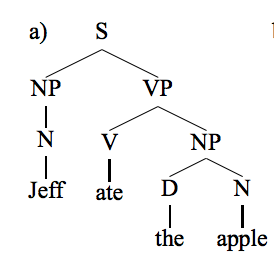
\includegraphics[width=0.3\textwidth]{shallow_parse_tree}
	\caption{Example of a Shallow Parse Tree \cite{zelenko2003kernel}}
	\label{fig:shallow_parse_tree}   
\end{figure} 
Kernels provide a similarity measure between two objects in some complex feature space. In contrast to feature based methods, kernel-based methods allow the original representation of the object to be retained, and the kernel function will work out the similarity measure. For instance, the sentence \emph{"Jeff ate the apple."} can represented as a shallow parse tree\cite{zelenko2003kernel}. The feature based methods would want to select features such as number of nodes, number of edges and directions of edges, whereas kernel based methods allows feeding the entire tree object into a tree kernel function K\cite{collins2001convolution}, and output the similarity measure between two trees $t_{1}$ and $t_{2}$ as $K(t_{1}, t_{2})$. Among various methods discussed above, we feel that \textbf{kernel based methods} can preserve the linguistically rich representations of sentences and has more flexibility as there are no manually encoded rules. The next chapter will discuss a graph kernel we chose for the relation extraction task in this project.

